\section{Decomposition and a Usable Rating Sheet}

A rating sheet makes a diagnosis inspectable. Its purpose is to connect each assessment with a task, boundary, and piece of evidence.

\subsection{Choose Units That Can Be Examined}

A unit should have an output that can be checked and an internally coherent process. Large differences in response time can signal a need to split it. A starting heuristic is
\begin{equation}
 \frac{\max_j\tau_j}{\min_j\tau_j}\leq\Lambda,
\end{equation}
with a declared $\Lambda$, perhaps ten. This does not guarantee that another subdivision is useless. The chosen grain must still preserve the mechanism being investigated.

Distinguish conversion units from interface units. A manufacturing step produces an item for the next step. Certification, procurement, access, and public participation connect the project to other systems. Both can change through better technology and organization.

\subsection{Ordinal Anchors}

The following anchors describe increasing constraint. They require task-specific criteria and evidence; they do not assign universal powers of ten.

\begin{table}[ht]
\centering\small
\begin{tabularx}{\textwidth}{@{}cYYY@{}}
\toprule
Grade & Resources & Time & Coupling\\
\midrule
0 & Small marginal demand within existing capacity & Effectively immediate for the task & Local change with few dependencies\\
1 & Available general equipment and supply & Short relative to the operating cycle & Known, standardized interfaces\\
2 & Dedicated equipment or materials & A material part of an operating cycle & Several interfaces need adaptation\\
3 & Significant supply, capital, or infrastructure commitments & A substantial planning or build cycle & Multiple teams or suppliers must coordinate\\
4 & Scarce inputs or major capacity changes & Long observation, replacement, or institutional process & Multiple organizations or jurisdictions interact\\
5 & A severe constraint under the specified boundary & Very long relative to the decision horizon & Extensive dependencies with difficult isolation\\
\bottomrule
\end{tabularx}
\caption{Illustrative ordinal anchors. A grade is an evidence-backed category, not a calibrated physical quantity.}
\end{table}

Grade zero still consumes material resources. Grade five does not establish impossibility. A physical conservation law can constrain a task without proving that every possible design has reached its limit.

Record uncertainty as an interval of plausible grades or a statement of missing evidence. A decimal grade creates no precision unless the scale has been calibrated.

For a defined dependency closure size $d_i$, one optional count-based binning is
\begin{equation}
 G_i=\min\left\{5,\left\lfloor\log_{10}(1+d_i)\right\rfloor\right\}.
\end{equation}
The closure definition matters more than the bin. Graph reachability, mandatory simultaneous modification, causal influence, and administrative contact are different relationships.

\subsection{Aggregate the Quantities Before the Grades}

Resources with matching units and boundaries can be added. Electricity, labor, cash, and materials need separate accounts or an explicit conversion. Averaging ordinal resource grades does not reconstruct total resource use.

Time depends on structure. For a serial chain with durations $t_i$,
\begin{equation}
 t_{\mathrm{serial}}=\sum_i t_i.
\end{equation}
For simultaneous tasks required before completion, elapsed time is their maximum. For a dependency graph it is the longest feasible path, under the stated resource and scheduling assumptions:
\begin{equation}
 t_{\mathrm{finish}}
 =\max_{p\in\mathcal P}\sum_{i\in p}t_i.
\end{equation}
A steady pipeline's throughput can be limited by its slowest stage. Throughput and first-item completion time are different quantities.

Amdahl's law supplies another conditional bound:
\begin{equation}
 S(n)=\frac{1}{s+(1-s)/n}\longrightarrow\frac1s,
 \qquad s\in(0,1].
\end{equation}
It assumes a fixed workload, serial fraction $s$, ideal parallelization of the remaining part, and omitted additional overhead \cite{amdahl1967validity}. An algorithm change can alter the workload or serial fraction.

Coupling needs a graph account. Report relevant degree and closure distributions, shared dependencies, cut sets, critical nodes, and possible cascade routes. A mean of coupling grades can conceal a decisive hub.

The familiar giant-component condition
\begin{equation}
 \frac{\langle k^2\rangle}{\langle k\rangle}>2
\end{equation}
belongs to a specified asymptotic random-graph setting with suitable regularity assumptions \cite{molloy1995critical}. It is not a universal threshold for directed, clustered, weighted industrial dependency networks. A connected component also does not imply simultaneous mandatory change.

Only after operational quantities have been defined and calibrated should they enter a quantitative model. A grade sheet remains useful without that step.

\subsection{What to Improve First}

Under a calibrated exponential model, the contribution $\alpha_c c$ can identify a large modeled constraint term. Choosing an intervention also needs the feasible reduction, cost, interactions, and risk.

For a small independent change with cost per unit reduction $\mu_c>0$, the ratio $\alpha_c/\mu_c$ compares modeled marginal log-cost benefit per spending unit. It does not establish absolute net benefit or select the best finite project when interventions interact.

If time is explicitly calibrated as $T=\log_{10}(\tau/\tau_0)$, then
\begin{equation}
 \ln\mathrm{De}=(\ln10)T
 -\ln\frac{\tau_{\mathrm{drive}}}{\tau_0}.
\end{equation}
This identity follows from that calibration. It cannot be inferred from a qualitative time grade.

\subsection{Worked Audit: A Low-Altitude Service}

Split a proposed service into cell production, pack and thermal system, airframe and rotors, flight control, terminals, operations and maintenance, airworthiness, airspace access, and the conditions under which the public will accept the service.

For each unit, collect actual durations, resource requirements, dependencies, validation evidence, and a responsible party. “Public acceptance takes ten years” is not an input one may simply declare. Identify the relevant population, decision, and observable acceptance condition.

A flight-control update can require substantial verification even when code changes quickly. Certification uses people, equipment, tests, and facilities. Airspace coordination uses infrastructure and operations. None is physically free because its output is a permission.

Create the dependency graph, then distinguish stages that run concurrently from those waiting on one another. A better battery may change aircraft performance, reserves, economics, and certification evidence together. The effect on launch time depends on the actual critical path.

If the next required authorization remains on that path, shortening an unrelated manufacturing step may not move the launch date. It can still reduce cost or improve later throughput. The method separates those outcomes.

\subsection{Five Comparison Questions}

\begin{table}[ht]
\centering\small
\begin{tabularx}{\textwidth}{@{}lYY@{}}
\toprule
Project & Resource and time questions & Dependency and evidence questions\\
\midrule
Inference service & Which capacity exists, and what does the whole request cost? & Which downstream actions can an output trigger?\\
Advanced fabrication & Which equipment, process, and yield constraints bind? & Which process changes need supplier and validation changes?\\
Low-altitude service & What mission energy, reserves, and facilities are required? & What evidence and authorizations govern the actual operation?\\
Gene-editing therapy & What delivery, production, exposure, and follow-up are required? & Which cell populations and clinical outcomes support the intended use?\\
Cement or steel decarbonization & What route, energy, feedstock, and replacement schedule are feasible? & How do plant, power, transport, product standards, and demand interact?\\
\bottomrule
\end{tabularx}
\caption{Comparable questions replace unsupported universal sector scores.}
\end{table}

The report should let another reader change an assessment by pointing to evidence. That is the rating sheet's central promise.

\begin{figure}[ht]
\centering
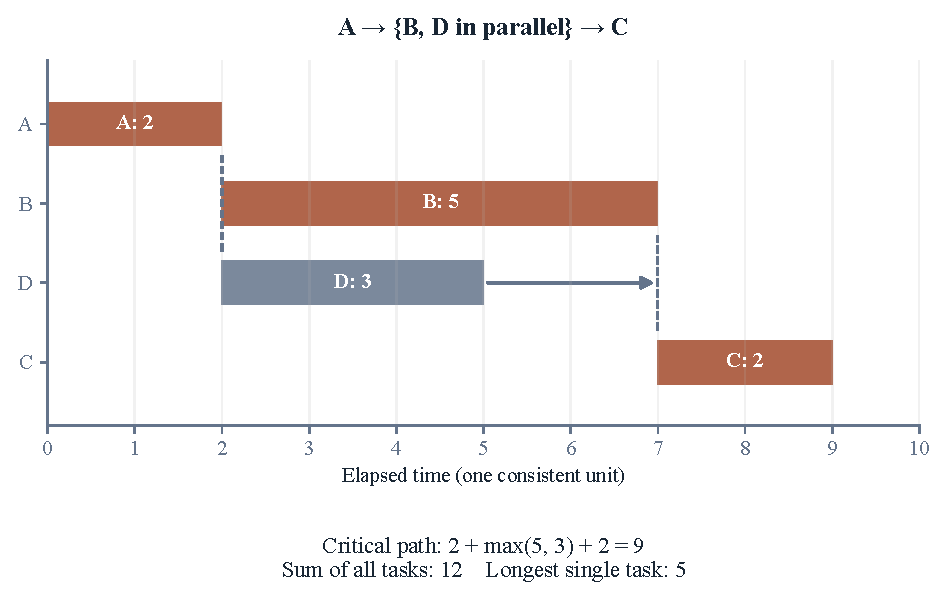
\includegraphics[width=\textwidth]{assets/critical-path.pdf}
\caption{A precedes parallel tasks B and D; C waits for both. Completion takes $2+\max(5,3)+2=9$, rather than the sum of all tasks (12) or the longest individual task (5). The critical path is A--B--C.}
\label{fig:mechanism-critical-path}
\end{figure}
